\section{Установка ownCloud Server в Debian GNU/Linux} \label{pril:c}

После успешного входа в систему, в первую очередь необходимо получить права суперпользователя\footnote{Пароль пользователя не отображается на экране во время набора} и добавить пользователя student в группу sudo:
\begin{lstlisting}
$ su -
Password: toor
# apt install sudo gnupg2 apt-transport-https
# usermod -a -G sudo student
\end{lstlisting}

Добавление репозитория и ключа для ownCloud Server:
\begin{lstlisting}
# wget -nv https://bit.ly/2I1dbjp -O Release.key
# apt-key add - < Release.key
OK
# echo deb http://download.owncloud.org\
> /download/repositories/production/Debian_9.0/ / > \
> /etc/apt/sources.list.d/owncloud.list
\end{lstlisting}

После добавления репозитория необходимо обновить список доступного в репозиториях ПО и запустить установку ownCloud Server (во время установки MySQL, установщик запросит пароль суперпользователя MySQL, он не обязательно должен совпадать с паролем пользователя root):
\begin{lstlisting}
# apt update
# apt install owncloud-files
...
New password for the MySQL "root" user: toor-mysql
Repeat password for the MySQL "root" user: toor-mysql
\end{lstlisting}

После того, как установщик скачал и установил все необходимые пакеты, можно проверить корректность установки, зайдя по адресу \texttt{http://192.168.0.102/owncloud/}, \\
где \texttt{192.168.0.102} "--- IP-адрес сервера (виртуальной машины).

Приложение предлагает использовать базу данных SQLite\footnote{Если возникли сложности с конфигурацией MySQL, то в качестве альтернативы можно использовать SQLite} по умолчанию, мы для примера будем использовать MySQL:
\begin{lstlisting}
# mysql -uroot -ptoor-mysql
mysql> CREATE DATABASE owncloudDB;
mysql> CREATE USER "owncloud-web"@"localhost" \
    -> IDENTIFIED BY "owncloud-passwd";
mysql> GRANT ALL PRIVILEGES ON owncloudDB.* \
    -> TO "owncloud-web"@"localhost";
mysql> FLUSH PRIVILEGES;
mysql> quit
\end{lstlisting}

После создания базы данных, необходимо обновить страницу приложения, настроить параметры базы данных и установить данные аккаунта администратора ownCloud (рис.~\ref{pic:db-own}).

\begin{figure}[ht]
    \centering
    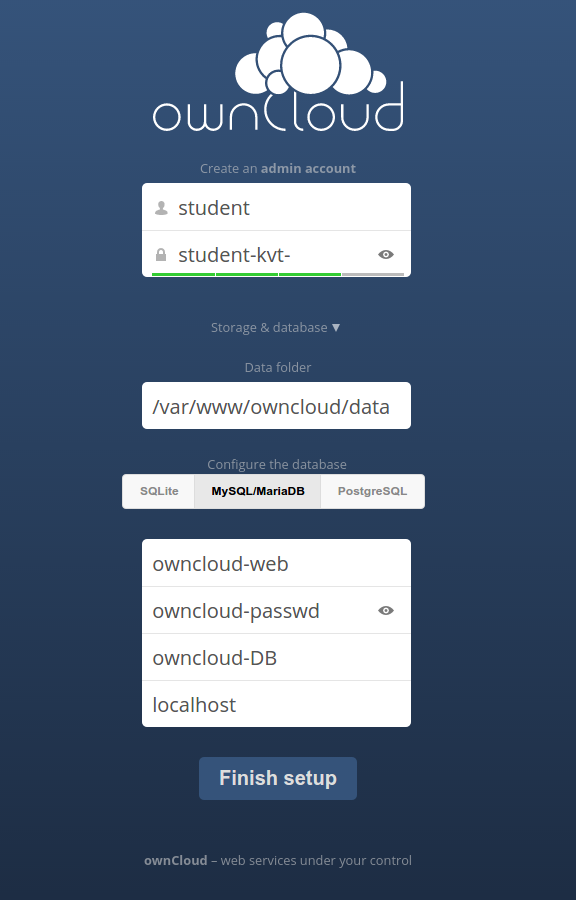
\includegraphics[width=0.8\linewidth]{Screenshot-2-owncloud}
    \caption{Параметры БД и аккаунта администратора}\label{pic:db-own}
\end{figure}

После нажатия клавиши <<Finish Setup>> база данных и пользовательские настройки успешно подключаются к ownCloud (рис.~\ref{pic:interface-own}).

\begin{figure}[ht]
    \centering
    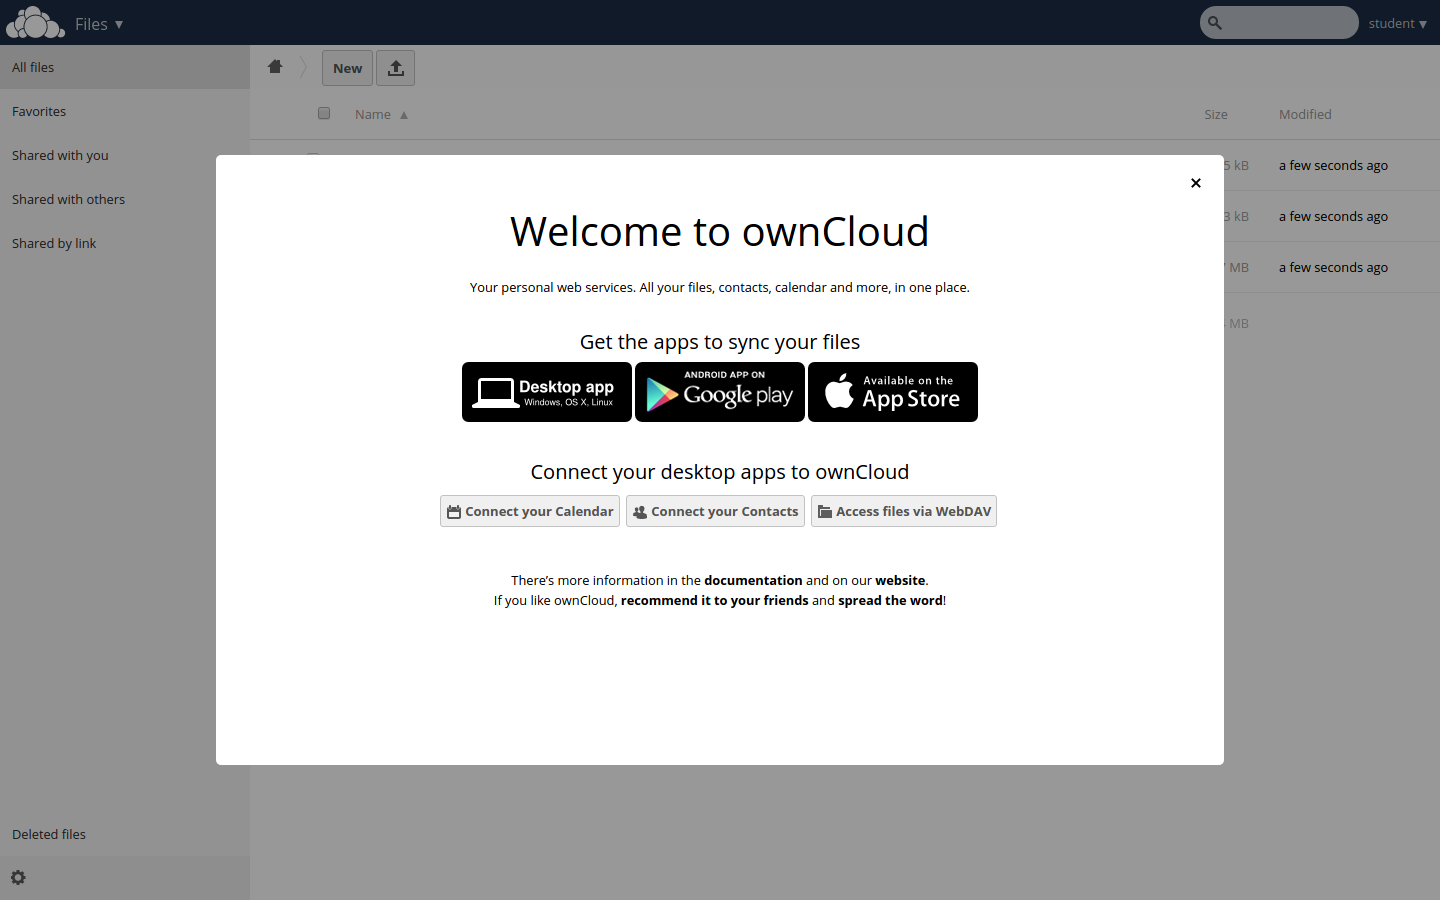
\includegraphics[width=\linewidth]{Screenshot-3-owncloud}
    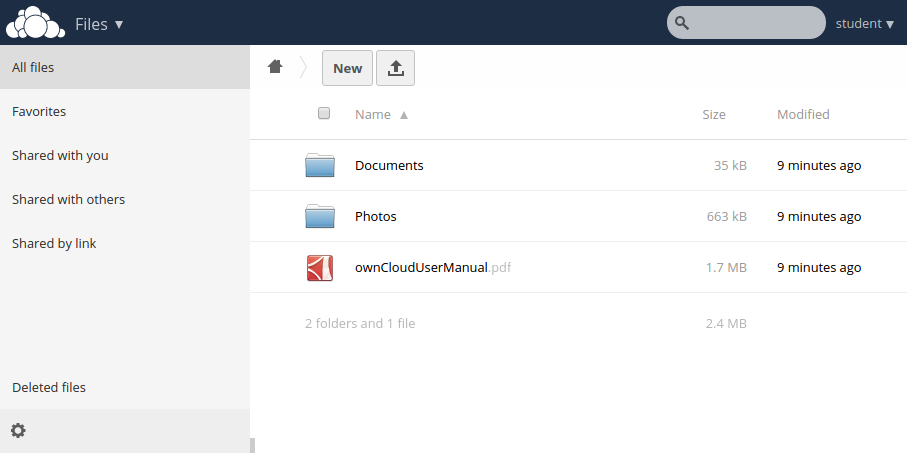
\includegraphics[width=\linewidth]{Screenshot-4-owncloud}
    \caption{Первый вход в ownCloud и интерфейс приложения}\label{pic:interface-own}
\end{figure}

\clearpage
